\documentclass{article}
\usepackage{tikz}

\begin{document}

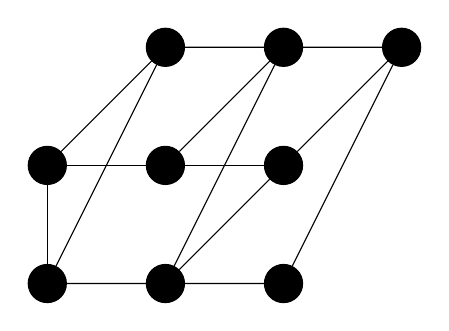
\begin{tikzpicture}[scale=1.5]
    % Define the nodes
    \node (1) at (0,0) [draw,circle,inner sep=2pt,fill] {1};
    \node (2) at (0,-1) [draw,circle,inner sep=2pt,fill] {2};
    \node (3) at (1,1) [draw,circle,inner sep=2pt,fill] {3};
    \node (4) at (1,0) [draw,circle,inner sep=2pt,fill] {4};
    \node (5) at (1,-1) [draw,circle,inner sep=2pt,fill] {5};
    \node (6) at (2,1) [draw,circle,inner sep=2pt,fill] {6};
    \node (7) at (2,0) [draw,circle,inner sep=2pt,fill] {7};
    \node (8) at (2,-1) [draw,circle,inner sep=2pt,fill] {8};
    \node (9) at (3,1) [draw,circle,inner sep=2pt,fill] {9};

    % Draw the edges
    \draw (1) -- (2);
    \draw (1) -- (3);
    \draw (1) -- (4);
    \draw (2) -- (3);
    \draw (2) -- (5);
    \draw (3) -- (6);
    \draw (4) -- (6);
    \draw (4) -- (7);
    \draw (5) -- (6);
    \draw (5) -- (7);
    \draw (5) -- (8);
    \draw (6) -- (9);
    \draw (7) -- (9);
    \draw (8) -- (9);

    % Add labels if needed
    % \node at (0.5,0.5) {$\gamma(G)=\overline{\gamma}(G)=3$};
    % \node at (0.5,-0.5) {$d_0(G)=5 > \overline{\gamma}(G)+1$};
\end{tikzpicture}

\end{document}